\section{System implementation} 
%3-5 pages
\subsection{Loading and preprocessing MNIST data}
The MNIST dataset is loaded in the function \code{get\_data} in file \code{encoding.py} using the function \code{keras.datasets.mnist.load\_data}. The images depicting the digits ``1'' and ``7'' are selected. Using the \code{get\_data} function, the desired number of samples can be specified and the distribution of both digits in the dataset can be balanced. The split ratio of the dataset in training and testing data can be chosen as well, with a default value of 0.8.
The images have a side length of 28\,px and are down-sampled using the \code{skimage.transform.resize} function in the function \code{down\_sample}. The default side length is 10\,px.
Then, the images are reshaped to an one-dimensional vector and normalized using the function \code{reshape\_and\_normalize}. The principle of the reshaping is illustrated in Figure \ref{fig:Objective-Scheme}.
%- with the argument \code{number} of the function \code{get\_data}, you can set the desired size of the sample-set.
%- Since the MNIST pool is slightly imbalanced (6742 ones vs 6265 sevens in the training split), taking all samples or choosing randomly would put the majority-class baseline towards 52.5\%. To prevent this inequality, the argument \code{balanced} enforces an equal count of every digit.
Furthermore, the energy in each image vector can be normalized in the function \code{get\_data} by dividing it by its norm.

\subsection{Linear Regression}
The linear regression is implemented using the Moore-Penrose pseudoinverse in the function \code{linear\_regression} in \code{baseline.py} (see Fig. \ref{code:lin-reg}).
Based on predicted labels \code{y\_pred} and the true labels, the confusion matrix and the accuracy for the binary classification are calculated.

\begin{figure}[H]
\centering
\begin{minted}
[
frame=none,
framesep=2mm,
baselinestretch=1.2,
bgcolor=codeyellow,
fontsize=\footnotesize,
linenos
]{python}
F = np.vstack([np.ones(len(X_train.T)), X_train]).T
theta = np.linalg.pinv(F) @ y_train

y_pred = theta[0] + np.sum(theta[1:] * X_test.T, axis = 1)
y_pred_label = (y_pred >= 0.5).astype(np.float64)
\end{minted}
\caption{Excerpt from function \code{linear\_regression} in \code{baseline.py}.}\label{code:lin-reg}
\end{figure}

\subsection{Optical Machine Learning}
\subsubsection{Encoding}
To encode information optically, we use the electromagnetic wave propagating through the wave-guide channels of the \gls{mzi} mesh. 
Since Maxwell's equations couple the electric and magnetic fields, it is sufficient to describe the wave by one of them, and therefore we work with the electric field throughout. 
For a monochromatic wave of angular frequency $\omega$ propagating along the waveguide axis with wave vector $\vec{k}$, the field in mode $j$ can be written as:
\begin{align*}
    E_j(\vec r, t) = A_j(\vec r)\, e^{i(\vec k \cdot \vec r + \omega t)}.
\end{align*}
Here we consider only a single scalar component of the field with amplitude $A_j$, omitting the vector character.
This is justified since we assume that all channels carry the same guided mode with a fixed polarisation.
For an uniform chip architecture, the channels acquire the exact same phase by propagating along the optical axis. Since the information is carried by the relative differences between the channels, we express the relevant components by 
\begin{align*}
    \mathbf{E}(\vec{r}, t) = e^{i(\vec{k} \cdot \vec{r} +\omega t)}
    \begin{pmatrix}
        A_1(\vec r)\, e^{i\varphi_1} \\ \vdots \\ A_m(\vec r)\, e^{i\varphi_m}
    \end{pmatrix},
\end{align*}
where $\varphi_j$ represents the initial phase given to the electric field in mode $j$.
The state of the system is therefore fully described by this vector of complex amplitudes, which is the quantity propagated in our simulation.
\\
The pixel values $V(x,y)$ of an image are imprinted on this field by modulating either the amplitudes $A_j$ or the initial phases $\varphi_j$ (see Fig. \ref{code:encoding}).
When applying amplitude encoding, the normalized pixel values are mapped onto the field
amplitudes while the phase is kept constant, with $E_j = \theta \, V_j$ and $\varphi_j = 0$.
%\begin{align*}
%    E_j = \theta \, V_j , \qquad \varphi_j = 0.
%\end{align*}
Phase encoding is an alternative in which the pixel values are mapped onto $\varphi_j$ at constant amplitude.
The hyperparameter $\theta$ is controlling the encoding strength.
%, is discussed as an alternative in Section~\ref{sec:AmplitudeEncoding}.

\begin{figure}[H]
\centering
\begin{minted}
[
frame=none,
framesep=2mm,
baselinestretch=1.2,
bgcolor=codeyellow,
fontsize=\footnotesize,
linenos
]{python}
def amplitude_encoding(image, theta_enc=1):
    """Encode image information in amplitude of electric field."""
    return (image * theta_enc).astype(complex)

def phase_encoding(image, theta_enc=1):
    """Encode pixel values in the phase, constant amplitude."""
    return np.exp(1j * theta_enc * np.pi * image)
\end{minted}
\caption{Excerpt from \code{encoding.py} showing the functions \code{amplitude\_encoding} and \code{phase\_encoding}.}\label{code:encoding}
\end{figure}

\subsubsection{Processing}
The processing is done by the \glspl{mzi} in the mesh, that can be set to perform any unitary transformation on the electric fields in each channel \cite{reckExperimentalRealizationAny1994}.
Consisting of an arrangement of beam splitters $B$ and phase shifters $R$ (see Figure \ref{fig:MZI-Phase-shifter}), the \gls{mzi} implements any arbitrary Givens rotation $T=R_\phi B R_\theta B$:
\begin{align*}
    T=\frac{1}{2} \begin{pmatrix}
    e^{i\phi} & 0 \\
    0 & 1
    \end{pmatrix}\begin{pmatrix}
    1 & i \\
    i & 1
    \end{pmatrix}\begin{pmatrix}
    e^{i\theta} & 0 \\
    0 & 1
    \end{pmatrix}
    \begin{pmatrix}
    1 & i \\
    i & 1
    \end{pmatrix}.
\end{align*}
Permutating their placements in the mesh along the layers allowing mixing between all channels, builds the \gls{oiu} that can form any unitary operation.
Applying these rotations block-wise to their respective channels, this yields the transfer-matrix of layer $L$, allowing the full propagation by matrix multiplication.
\begin{align}
    \mathbf{E_{out}}=\hat{W}_L\hat{W}_{L-1}...\hat{W}_1\mathbf{E_{in}}=\hat{W}\mathbf{E_{in}}.
    \label{eq:layerwisepropagation}
\end{align}
Note that a layer here refers to the depth of one \gls{mzi} (2 beam splitters and 2 phase shifters) and is not to be confused with the definition of one layer for the adjoint-based backpropagation. There each layers is representing one tunable parameter (1 beam splitter and 1 phase shifter).

Accordingly, the transfer matrices are calculated using functions \code{beamsplitter}, \code{phase\_shift} and \code{U} (see Fig. \ref{code:transfer-matrices}).
Additionally, two functions \code{U\_theta} and \code{U\_phi} are defined which allow a separate calculation of the transfer matrices for each combination of a phase shifter and beam splitter separately for the gradient-descent algorithm.

\begin{figure}[H]
\centering
\begin{minted}
[
frame=none,
framesep=2mm,
baselinestretch=1.2,
bgcolor=codeyellow,
fontsize=\footnotesize,
linenos
]{python}
def beamsplitter(eta=1.0):
    """Transfer matrix of a beamsplitter with power transmission eta."""
    B_ideal = (1/np.sqrt(2)) * np.array([[1, 1j],
                                         [1j, 1]], dtype=np.complex128)
    return np.sqrt(eta) * B_ideal

def phase_shift(alpha): 
    """Transfer matrix to apply a phase shift to upper mode."""
    return np.array([[np.exp(1j*alpha), 0],
                     [0, 1]], dtype=np.complex128)

def U(theta, phi, eta=1.0):
    """Transfer matrix of the MZI with phase shifts theta and phi. 
    eta: Power transmission per beamsplitter. Two beamsplitters per MZI."""
    B = beamsplitter(eta)
    return phase_shift(phi) @ B @ phase_shift(theta) @ B
\end{minted}
\caption{Excerpt from \code{mesh.py} showing the functions \code{beamsplitter}, \code{phase\_shift} and \code{U}.}\label{code:transfer-matrices}
\end{figure}

The class \code{MZIMesh} is a central part of the processing (see Fig. \ref{fig:class-MZIMesh}). It allows the definition of the chip structure. 
The implemented options include a rectangular and a triangular mesh of \gls{mzi}s.
According to \citeauthor{paiMatrixOptimizationUniversal2019a}, convergence can be vastly accelerated by using the correct initialization. The ``Haar initialization'' introduced in \cite{paiMatrixOptimizationUniversal2019a}, is based on globally approximating a uniformly random unitary matrix rather than just randomizing individual components. Thus, position-dependent \gls{mzi} split ratios form a global Haar-random matrix, ensuring that input light is evenly distributed across all spatial modes.
The code for the generation of the rectangular mesh is shown in Figure \ref{code:rect-mesh} as an example.
Parameters, like the values of \code{theta} and \code{phi} for each phase shifter are stored separately. 

\begin{figure}[H]
    \centering
    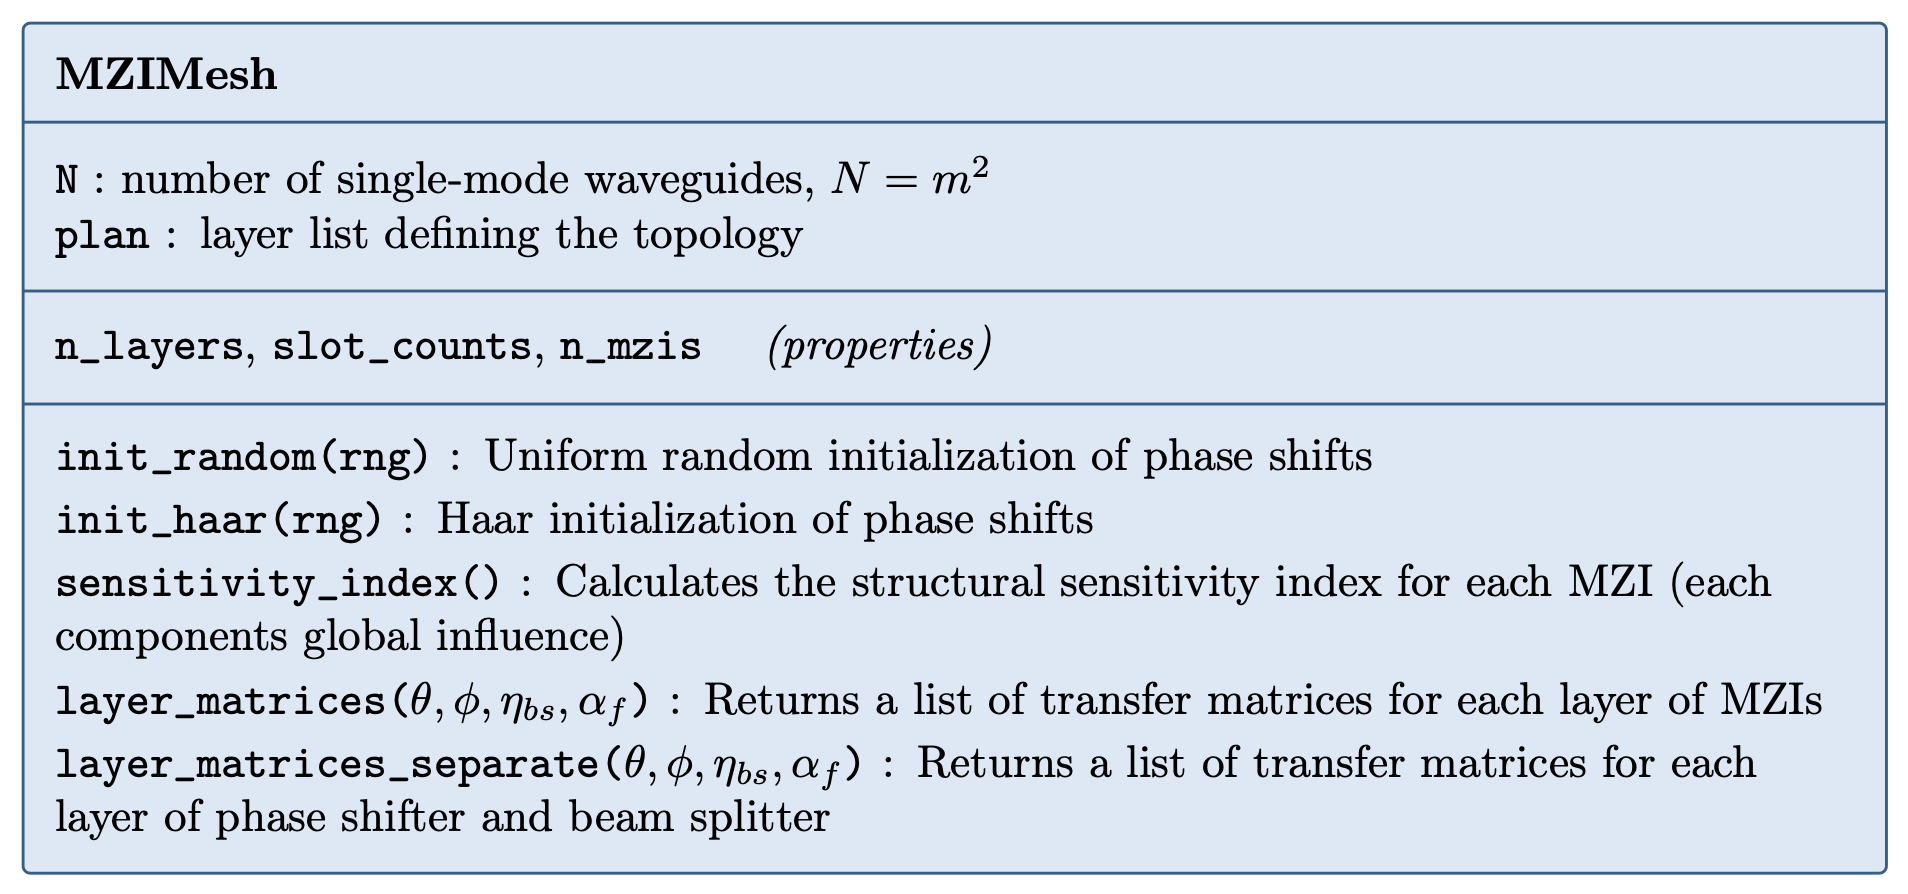
\includegraphics[width=0.7\linewidth]{images/main_classdiagram_mesh.png}
    \caption{Class diagram for class MZIMesh from mesh.py}
    \label{fig:class-MZIMesh}
\end{figure}

\begin{figure}[H]
\centering
\begin{minted}
[
frame=none,
framesep=2mm,
baselinestretch=1.2,
bgcolor=codeyellow,
fontsize=\footnotesize,
linenos
]{python}
def plan_rectangular(N, L):
    """Clements / rectangular mesh: L Layers, with alternating offset 0 and 1.
    Universal for L = N. Returns: list of ("mzi", ks)."""
    plan = []
    for l in range(L):
        start = l % 2
        ks = list(range(start, N - 1, 2))
        plan.append(("mzi", ks))
    return plan
\end{minted}
\caption{Excerpt from \code{mesh.py} showing the function \code{plan\_rectangular}.}\label{code:rect-mesh}
\end{figure}

The functions which are most relevant for the propagation of the electric field in the chip are summarized in Figure \ref{code:propagation}.
The function \code{forward} returns the electric field at the output ports of the chip on the right, when an electric field has entered through the input ports on the left, while the function \code{backward} gives the output field for the reverse propagation direction from the right to the left.
The output of the forward propagation is calculated by applying the transfer matrix $\hat{W}_L$ of each layer which are stored in \code{layers} to the incoming electric field vector.
For the backward propagation the transfer matrices are transposed and their order is reversed, then they are applied to the electric field vector incoming from the right.

\begin{figure}[H]
\centering
\begin{minted}
[
frame=none,
framesep=2mm,
baselinestretch=1.2,
bgcolor=codeyellow,
fontsize=\footnotesize,
linenos
]{python}
def forward(E_in, layers):
    """Forward propagation through given layers."""
    for Ml in layers:
        E = Ml @ E
    return E

def backward(lam_out, layers):
    """Backward propagation through reversed layers."""
    return forward(lam_out, adjoint_layers(layers))

def adjoint_layers(layers):
    """Transposing layers and reversal of their order."""
    return [Ml.T for Ml in reversed(layers)]
\end{minted}
\caption{Shortened excerpt from \code{processing.py} showing the functions \code{forward}, \code{backward} and \code{adjoint\_layers} which are relevant for the electric field propagation through the chip.}\label{code:propagation}
\end{figure}

\subsubsection{Decoding}
The detected intensity is calculated as the absolute squared value of the electrical field for each output:
$I_n=|E_{out,n}|^2=E_{out,n}\cdot E_{out,n}^*$.
Two specific output ports are assigned to digits ``1'' and ``7'' respectively.
The digit assigned to the port with the higher intensity is returned as the predicted label. This is implemented in the functions \code{detection} and \code{\_detector\_scores} in \code{decoding.py}.

\subsubsection{Gradient-Descent Training Through Adjoint-based Backpropagation}
Conventional backpropagation operates on a known computational graph and requires the transpose of each weight matrix to be available as an explicit numerical object. 
In our system the weights are not numbers stored in memory but the phase settings of the \glspl{mzi}, and the linear operation they implement is a propagating optical field.
What is therefore needed is a formulation of the same gradient in terms of the physical parameters of the device.

The \gls{avm} provides exactly this formulation. 
It originates in the calculus of variations and was later adapted to engineering sensitivity analysis. 
Today it is a standard tool of photonic inverse design
\cite{gilesIntroductionAdjointApproach2000, veronisMethodSensitivityAnalysis2004, moleskyInverseDesignNanophotonics2018}.
Its key result is that the derivative of a scalar figure of merit with respect to all design parameters follows from only two field solutions. 
The first is the original field, driven by the physical input source. 
The second is an adjoint field, driven by a source that encodes the error at the output \cite{hughesAdjointMethodInverse2018}. 
The gradient with respect to an individual parameter is then given by the local overlap of these two fields at its position.
For the calculation of the gradient, we use the following equation, which is derived in appendix \ref{appendix:derivation}:
\begin{align}
    \frac{\mathrm{d}\mathcal{L}}{\mathrm{d}p}
    = -2\,\Im\left\{ A_p\,A_p^{\mathrm{adj}} \right\}
    \label{eq:final1}
\end{align}
%\paragraph{Algorithmic Implementation in \code{trainer} class}\mbox{}\\
Summarizing this derivation, that is specifically matched to our system, we get the following practical procedure for our training:
%(In our software based simulation, we...)
\begin{enumerate}
    \item Propagating the input field $\mathbf{E}_{in}$ (encoded MNIST data) using forward propagation according to equation \eqref{eq:layerwisepropagation}. After every phase shifter ($\phi$ and $\theta$), the electrical field in that channel is stored in a list.
    \item Decoding the output and calculating the loss for the chosen cost function. Determining the adjoint vector for the backpropagation.
    \item Propagating the adjoint field using backward propagation through the transposed layer transfer matrices. After every phase shifter ($\phi$ and $\theta$), the electrical field in that channel is stored in a list.
    \item Calculating the derivative of the loss with respect to each phase shifter using equation \eqref{eq:final1} by interfering the forward and backward propagated fields at each position.
    The parameters $\phi$ and $\theta$ are updated accordingly using gradient-descent.
\end{enumerate}

%\subsection{Zusammenfassung des Trainingsschritts}

%Ein vollständiger Gradientenschritt besteht damit aus vier Operationen:

%\begin{enumerate}
%  \item Propagation des kodierten Eingangsfeldes $\mathbf{E}_0$ durch das Mesh
%        gemäß \eqref{eq:layerwisepropagation} unter Speicherung der Feldamplituden nach jeder
%        Layer-Ebene.
%  \item Auswertung der Detektorintensitäten \eqref{eq:detection}, der
%        Kostenfunktion $\mathcal{L}$ und der adjungierten Quelle
%        \eqref{eq:adjointsource}.
%  \item Rückwärtspropagation der adjungierten Quelle durch die transponierten
%        Layer-Matrizen unter Speicherung der adjungierten Amplituden an
%        denselben Positionen.
%  \item Bildung des Überlapps \eqref{eq:gradient} für alle Phasenschieber
%        gleichzeitig und Aktualisierung der Parameter.
%\end{enumerate}

%Da Schritt~1 und Schritt~3 jeweils eine einzige Propagation durch das Netzwerk
%erfordern, ist der Aufwand pro Trainingsschritt unabhängig von der Zahl der
%trainierbaren Phasen --- gegenüber den eingangs genannten $2 \cdot 10^{4}$
%Propagationen einer Finite-Differenzen-Auswertung eine Reduktion um vier
%Größenordnungen.


%"1. Send in the original field amplitudes X l−1 and measure and store the intensities at each phase shifter.
%2. Send δl into the output ports and measure and store the intensities at each phase shifter.
%3. Compute the time-reversed adjoint input field amplitudes as in Eq. (25).
%4. Interfere the original and the time-reversed adjoint fields in the device, measuring again the resulting intensities at each phase shifter.
%5. Subtract the constant intensity terms from steps 1 and 2 and multiply by k2 0 to recover the gradient as in Eq. (23)."

%\subsubsection{Training Algorithm}
%\label{ssec:TrainingAlgorithm}
%Hier drauf eingehen, wie die Trainingsschritte in der Klasse \code{trainer} umgesetzt werden (Programmcode)
The class \code{trainer} is used for the training of the model, i.e. the optimization of the applied phase shifts.
The attributes and functions of the class are shown in the class diagram in Figure \ref{fig:class-trainer}. The algorithm of the function \code{fit} of the \code{trainer} class is depicted as a flowchart in Figure \ref{fig:training_flow}.
Figure \ref{code:gradient} shows the implementation of equation \eqref{eq:final1} for the calculation of the gradient at each phase shifter in function \code{gradient} in the code.

\begin{figure}[H]
    \centering
    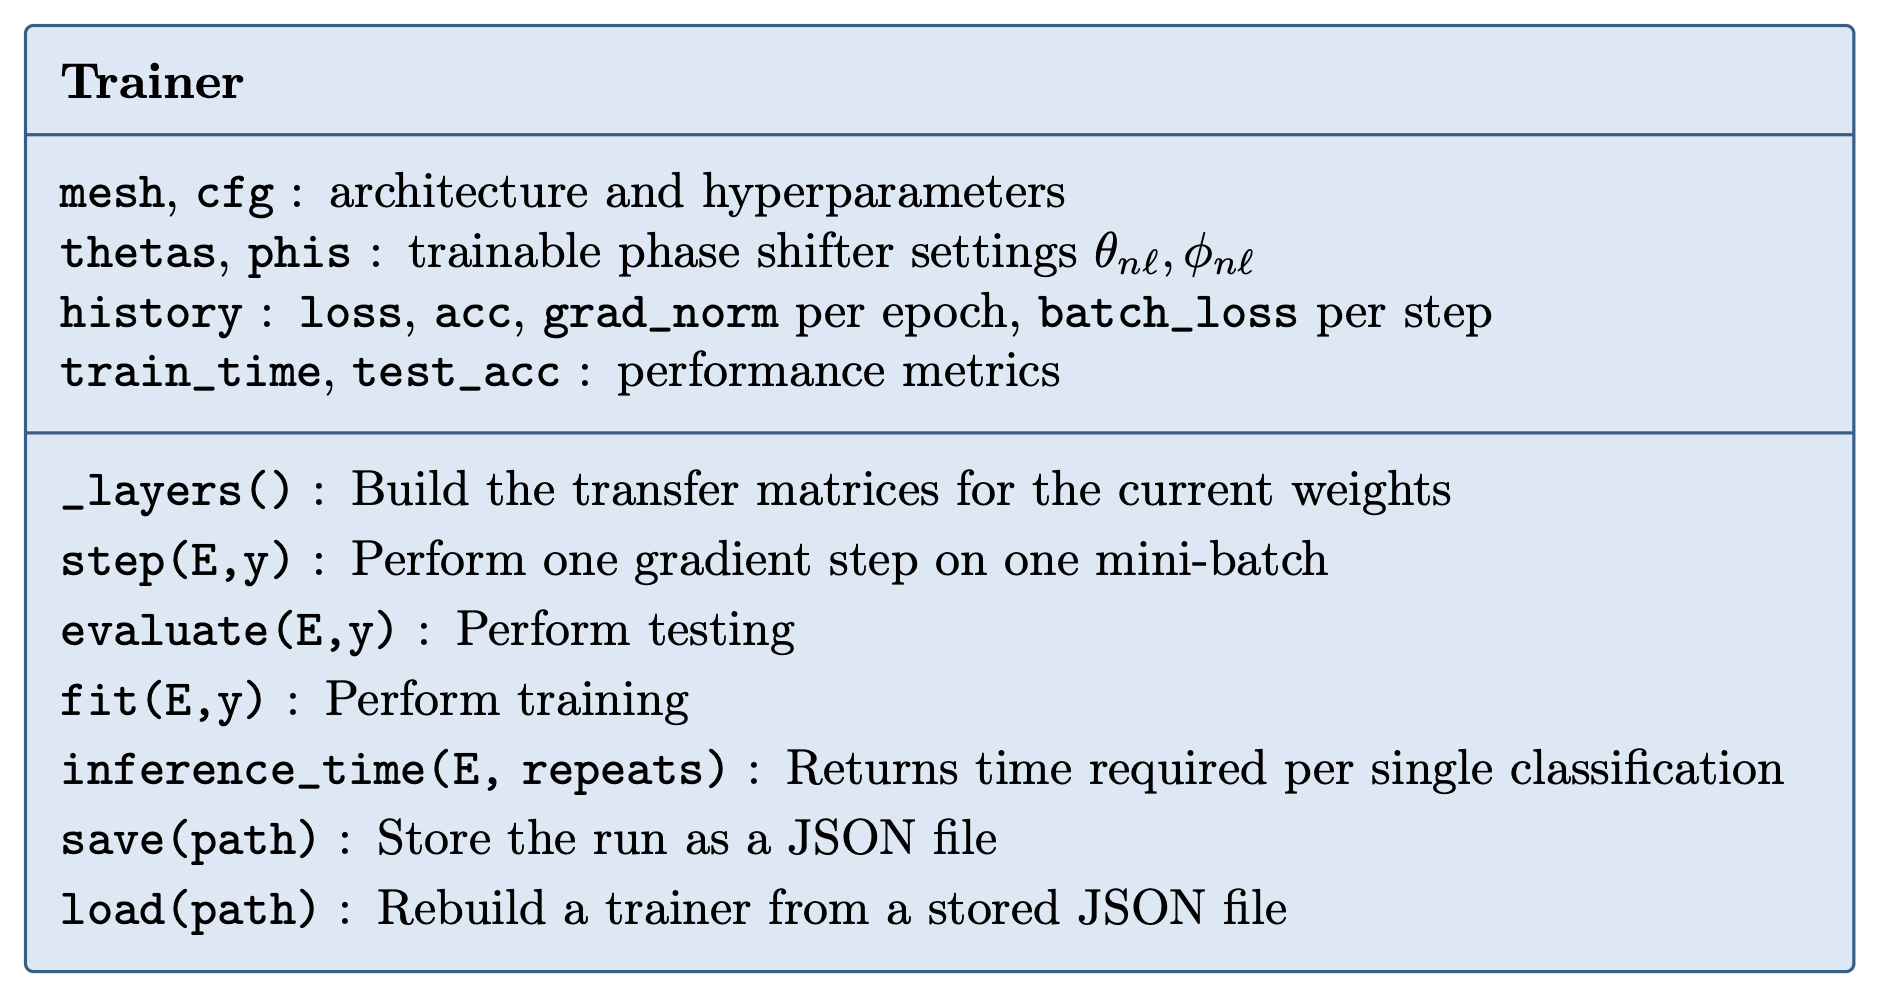
\includegraphics[width=0.7\linewidth]{images/main_classdiagram_trainer.png}
    \caption{Class diagram for \code{trainer} class from \code{trainer.py}.}
    \label{fig:class-trainer}
\end{figure}

\begin{figure}[H]
    \centering
    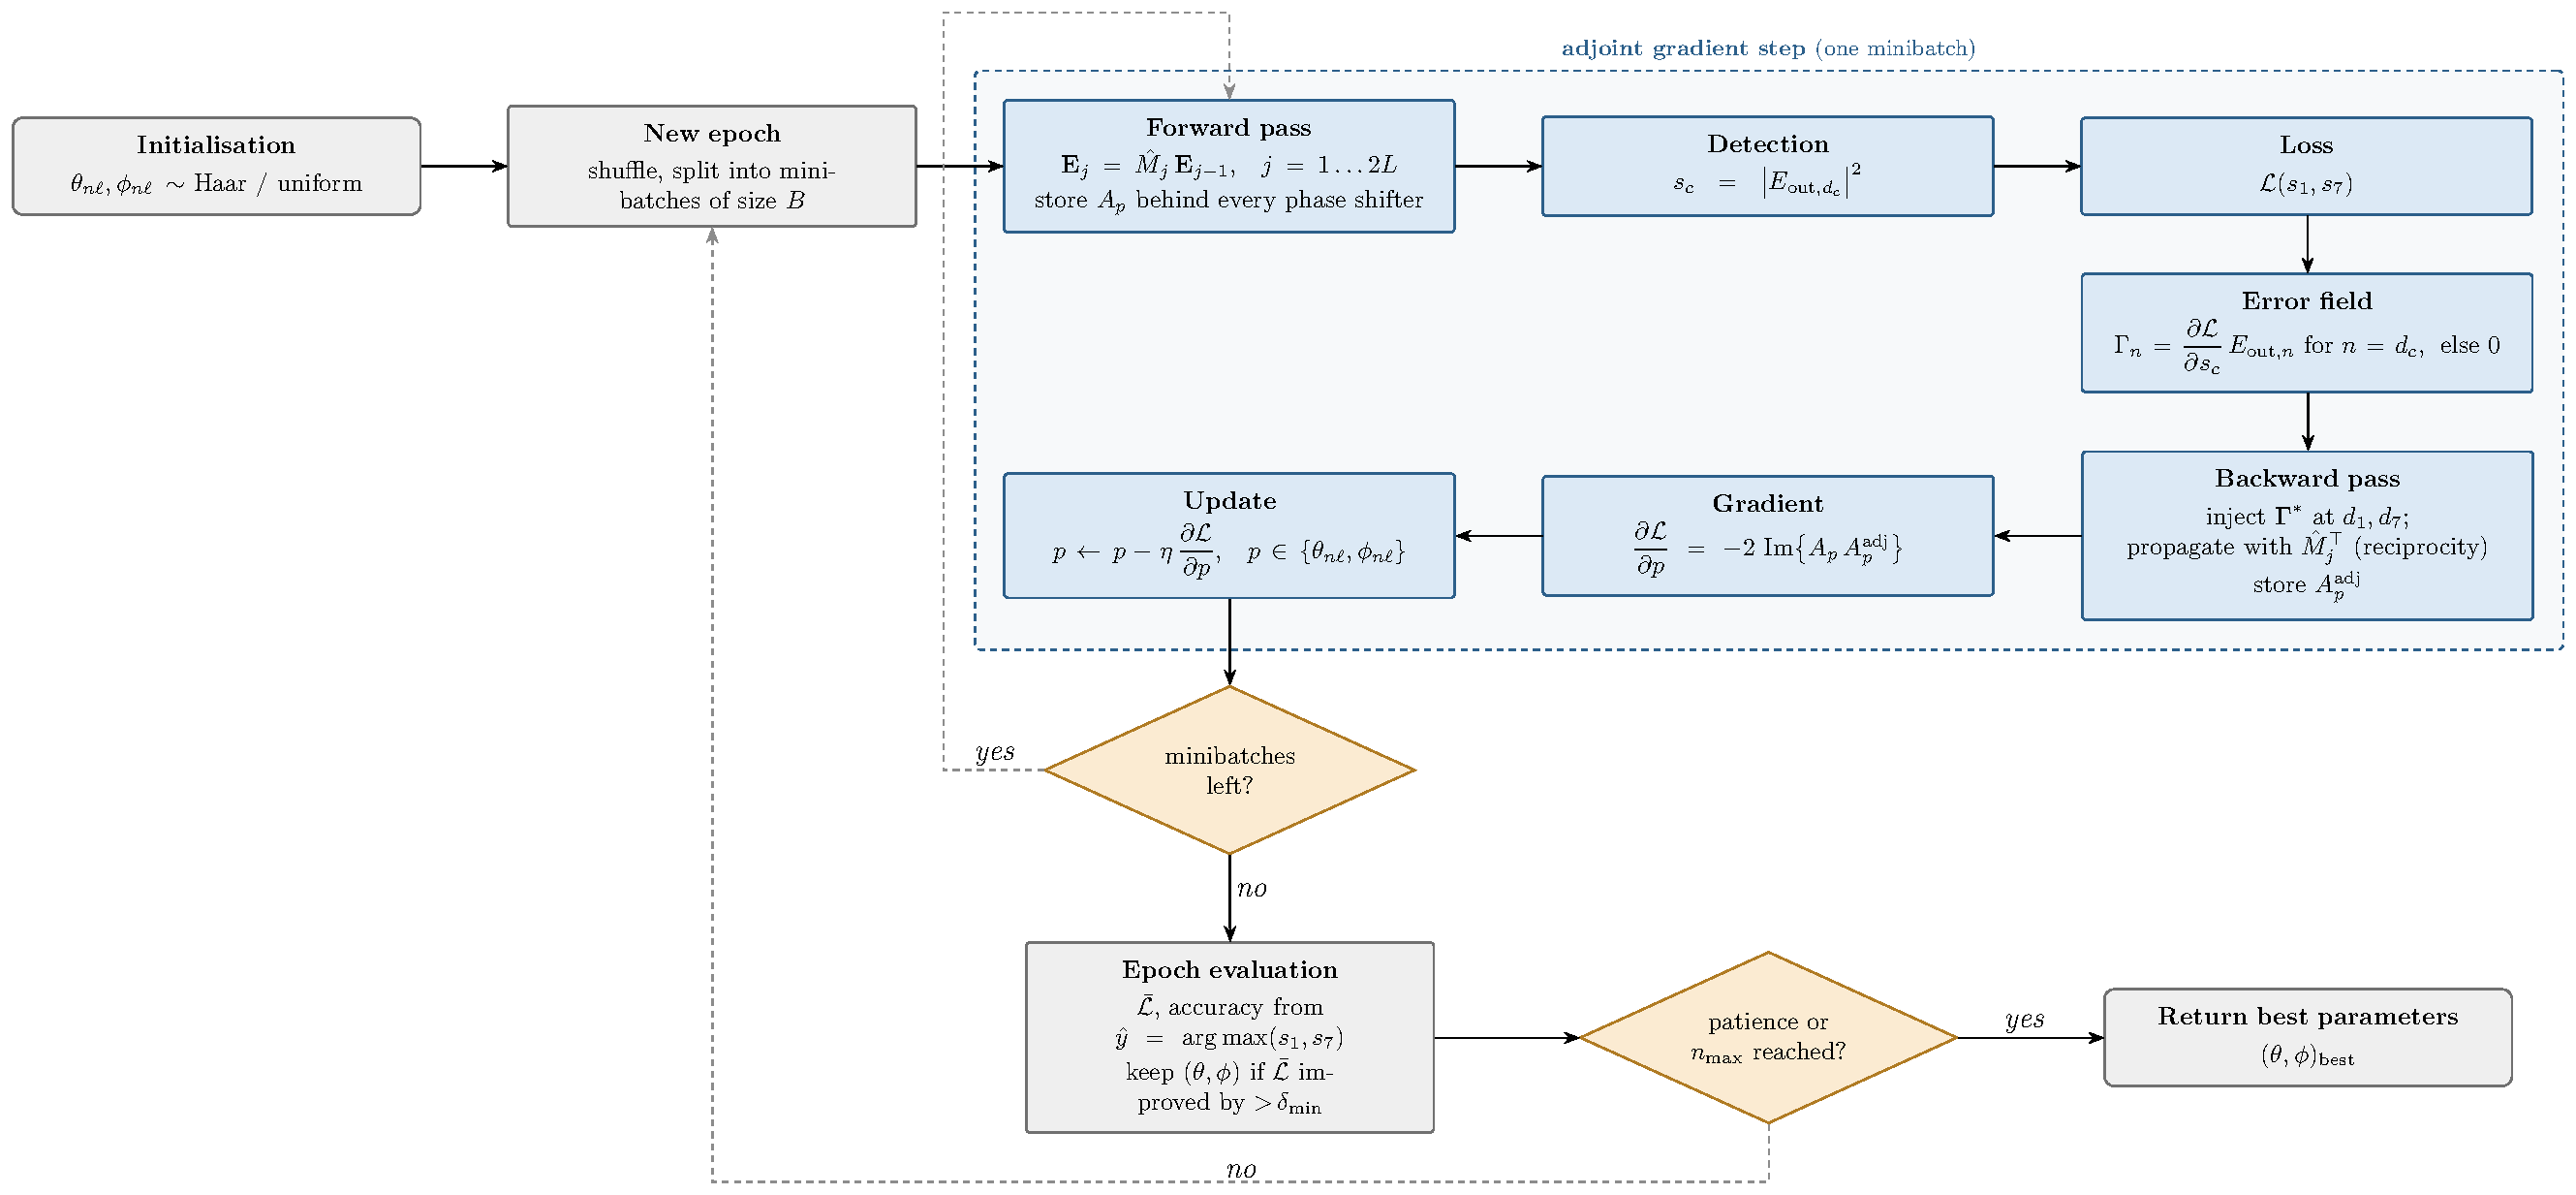
\includegraphics[width=\linewidth]{charts/trainer_algo_flowchart_horizontal.pdf}
    \caption{Flowchart of \code{fit}-algorithm in \code{trainer} class.}
    \label{fig:training_flow}
\end{figure}

%Conventional backpropagation operates on a known computational graph and requires the transpose of each weight matrix to be available as an explicit numerical object. In our system the weights are not numbers stored in memory but the phase settings of the \glspl{mzi} that are subject to drift.




\begin{figure}[H]
\centering
\begin{minted}
[
frame=none,
framesep=2mm,
baselinestretch=1.2,
bgcolor=codeyellow,
fontsize=\footnotesize,
linenos
]{python}
def gradient(fh, bh, plan):
    """Calculation of gradient for all values of theta and phi based on forward and backward
    propagating fields"""
    grad_th, grad_ph = [], []
    for l, (kind, ks) in enumerate(plan):
        gt = np.zeros(len(ks)); gp = np.zeros(len(ks))
        for i, k in enumerate(ks):
            # phase_shift applied to upper mode only
            gt[i] = -2*np.imag(np.sum(bh[2*l+1][k] * fh[2*l+1][k]))
            gp[i] = -2*np.imag(np.sum(bh[2*l+2][k] * fh[2*l+2][k]))
        grad_th.append(gt); grad_ph.append(gp)
    return grad_th, grad_ph
\end{minted}
\caption{Shortened excerpt from \code{processing.py} showing the function \code{gradient}.}\label{code:gradient}
\end{figure}

The loss function $\mathcal{L}(s_1, s_7)$ depends on the scores of the chosen detectors for the digits 1 ($s_1$) and 7 ($s_7$).
Two loss functions are implemented in \code{decoding.py}: mean square error (function \code{mse}) and softmax-cross-entropy (function \code{softmax\_ce}).
The mean squared error loss and its derivative with respect to the detector score can be defined as:
\begin{align*}
    \mathcal{L}_{\text{MSE}}(s_1, s_7) &= \sum_{c \in \{1,7\}} (s_c - t_c)^2 \text{ and }
    \frac{\partial \mathcal{L}_{\text{MSE}}}{\partial s_c} = 2(s_c - t_c).
\end{align*}

The softmax-cross-entropy loss and its derivative are given by:
\begin{align*}
    \mathcal{L}_{\text{CE}}(s_1, s_7) &= - \sum_{c \in \{1,7\}} t_c \log(p_c) \text{ and }
    \frac{\partial \mathcal{L}_{\text{CE}}}{\partial s_c} = p_c - t_c
    \text{ with }
    p_c = \frac{e^{s_c}}{e^{s_1} + e^{s_7}},
    %\label{eq:softmax}
\end{align*}
where $t$ is the target value.
